% Auto-generated by the analysis pipeline — do not edit
% y > 0: Overreacts  |  y < 0: Underreacts
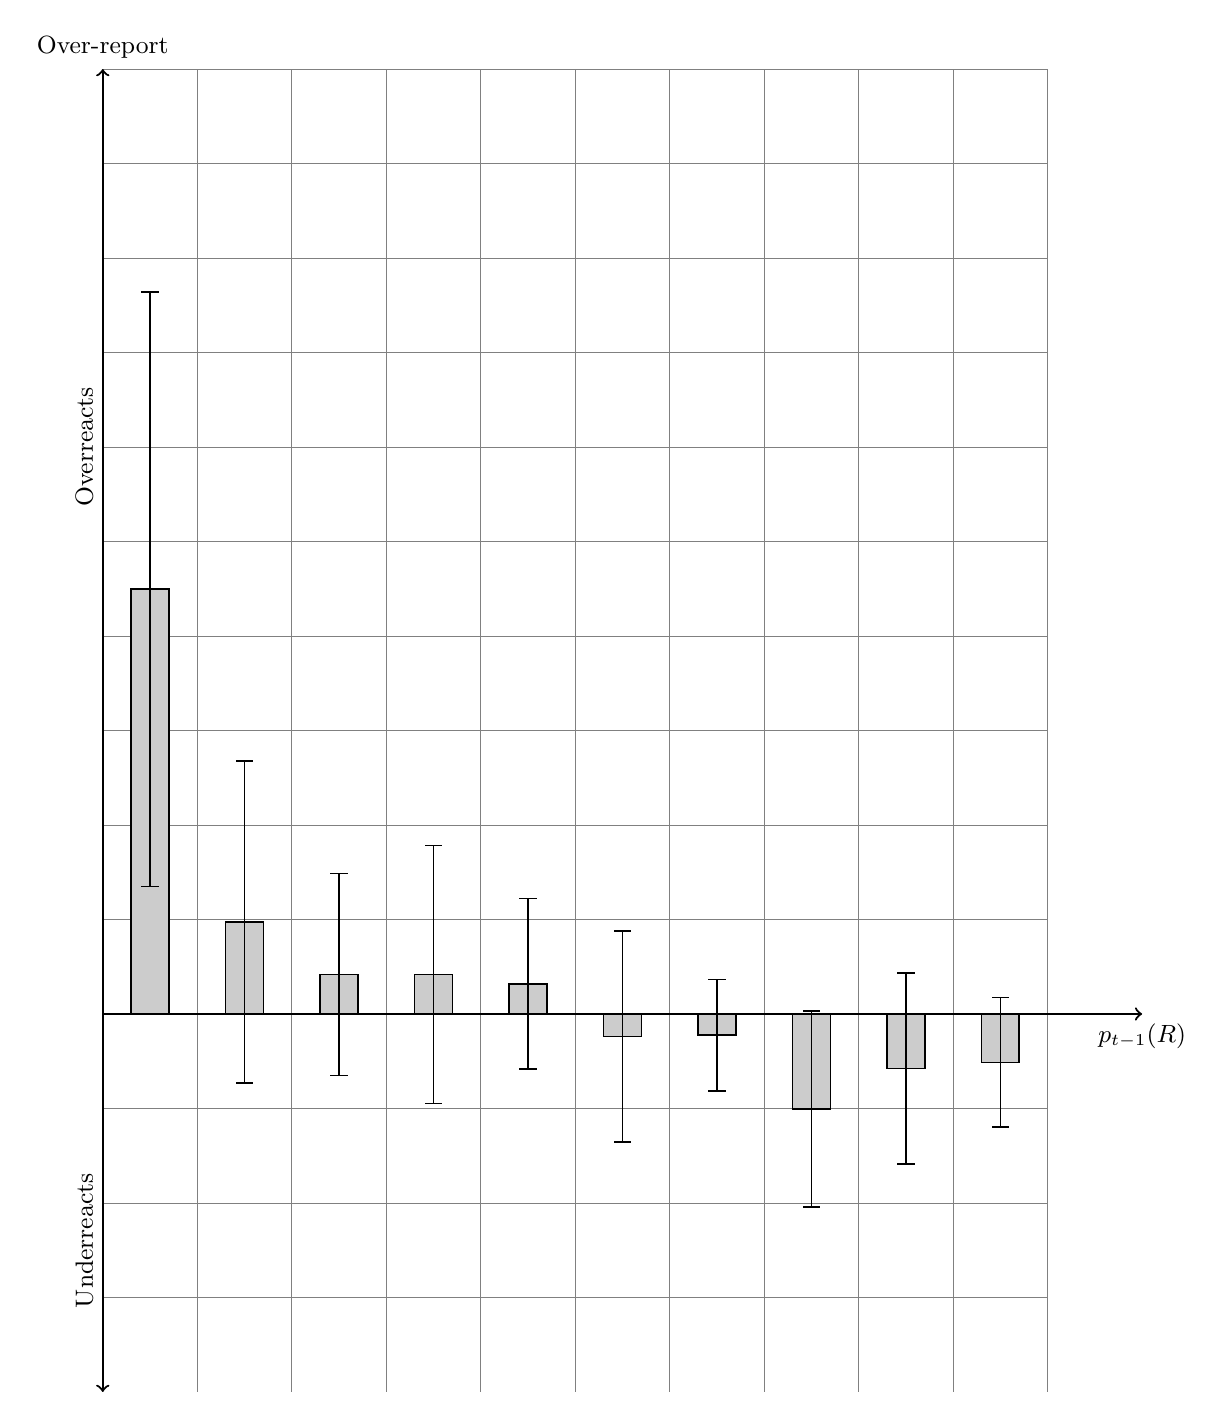
\begin{tikzpicture}[scale=12]
\draw[help lines,step=0.1] (0,-0.4) grid (1,1.0);
\filldraw[opaque,white!80!black] (0.03,0) rectangle (0.07,0.4496);
\draw[line width=0.6] (0.03,0) rectangle (0.07,0.4496);
\draw[line width=0.6,|-|] (0.05,0.1341) -- (0.05,0.7652);
\filldraw[opaque,white!80!black] (0.13,0) rectangle (0.17,0.0971);
\draw[line width=0.6] (0.13,0) rectangle (0.17,0.0971);
\draw[line width=0.6,|-|] (0.15,-0.0742) -- (0.15,0.2684);
\filldraw[opaque,white!80!black] (0.23,0) rectangle (0.27,0.0417);
\draw[line width=0.6] (0.23,0) rectangle (0.27,0.0417);
\draw[line width=0.6,|-|] (0.25,-0.0659) -- (0.25,0.1494);
\filldraw[opaque,white!80!black] (0.33,0) rectangle (0.37,0.0418);
\draw[line width=0.6] (0.33,0) rectangle (0.37,0.0418);
\draw[line width=0.6,|-|] (0.35,-0.0956) -- (0.35,0.1792);
\filldraw[opaque,white!80!black] (0.43,0) rectangle (0.47,0.0320);
\draw[line width=0.6] (0.43,0) rectangle (0.47,0.0320);
\draw[line width=0.6,|-|] (0.45,-0.0591) -- (0.45,0.1230);
\filldraw[opaque,white!80!black] (0.53,0) rectangle (0.57,-0.0239);
\draw[line width=0.6] (0.53,0) rectangle (0.57,-0.0239);
\draw[line width=0.6,|-|] (0.55,-0.1365) -- (0.55,0.0887);
\filldraw[opaque,white!80!black] (0.63,0) rectangle (0.67,-0.0223);
\draw[line width=0.6] (0.63,0) rectangle (0.67,-0.0223);
\draw[line width=0.6,|-|] (0.65,-0.0821) -- (0.65,0.0375);
\filldraw[opaque,white!80!black] (0.73,0) rectangle (0.77,-0.1004);
\draw[line width=0.6] (0.73,0) rectangle (0.77,-0.1004);
\draw[line width=0.6,|-|] (0.75,-0.2049) -- (0.75,0.0042);
\filldraw[opaque,white!80!black] (0.83,0) rectangle (0.87,-0.0577);
\draw[line width=0.6] (0.83,0) rectangle (0.87,-0.0577);
\draw[line width=0.6,|-|] (0.85,-0.1596) -- (0.85,0.0442);
\filldraw[opaque,white!80!black] (0.93,0) rectangle (0.97,-0.0512);
\draw[line width=0.6] (0.93,0) rectangle (0.97,-0.0512);
\draw[line width=0.6,|-|] (0.95,-0.1208) -- (0.95,0.0184);
\draw[line width=0.8,->]  (0,0) -- (1.1,0) node[below] {\small{$p_{t-1}(R)$}};
\draw[line width=0.8,<->] (0,-0.4) -- (0,1.0) node[above] {\small{Over-report}};
\draw (0,0.60) node[above,rotate=90] {\small{Overreacts}};
\draw (0,-0.24) node[above,rotate=90] {\small{Underreacts}};
% ADD THEORY CURVE BELOW
\end{tikzpicture}
